\documentclass[bachelor, och, referat]{shiza}
% параметр - тип обучения - одно из значений:
%    spec     - специальность
%    bachelor - бакалавриат (по умолчанию)
%    master   - магистратура
% параметр - форма обучения - одно из значений:
%    och   - очное (по умолчанию)
%    zaoch - заочное
% параметр - тип работы - одно из значений:
%    referat    - реферат
%    coursework - курсовая работа (по умолчанию)
%    diploma    - дипломная работа
%    pract      - отчет по практике
% параметр - включение шрифта
%    times    - включение шрифта Times New Roman (если установлен)
%               по умолчанию выключен
\usepackage{subfigure}
\usepackage{tikz,pgfplots}
\pgfplotsset{compat=1.5}
\usepackage{float}

%\usepackage{titlesec}
\setcounter{secnumdepth}{4}
%\titleformat{\paragraph}
%{\normalfont\normalsize}{\theparagraph}{1em}{}
%\titlespacing*{\paragraph}
%{35.5pt}{3.25ex plus 1ex minus .2ex}{1.5ex plus .2ex}

\titleformat{\paragraph}[block]
{\hspace{1.25cm}\normalfont}
{\theparagraph}{1ex}{}
\titlespacing{\paragraph}
{0cm}{2ex plus 1ex minus .2ex}{.4ex plus.2ex}

% --------------------------------------------------------------------------%


\usepackage[T2A]{fontenc}
\usepackage[utf8]{inputenc}
\usepackage{graphicx}
\graphicspath{ {./images/} }
\usepackage{tempora}

\usepackage[sort,compress]{cite}
\usepackage{amsmath}
\usepackage{amssymb}
\usepackage{amsthm}
\usepackage{fancyvrb}
\usepackage{listings}
\usepackage{listingsutf8}
\usepackage{longtable}
\usepackage{array}
\usepackage[english,russian]{babel}

%\usepackage[colorlinks=true]{hyperref}
\usepackage{url}

\usepackage{underscore}
\usepackage{setspace}
\usepackage{indentfirst} 
\usepackage{mathtools}
\usepackage{amsfonts}
\usepackage{enumitem}
\usepackage{tikz}
\newcommand{\eqdef}{\stackrel {\rm def}{=}}
\newcommand{\specialcell}[2][c]{%
\begin{tabular}[#1]{@{}c@{}}#2\end{tabular}}

\renewcommand\theFancyVerbLine{\small\arabic{FancyVerbLine}}

\newtheorem{lem}{Лемма}

\begin{document}

% Кафедра (в родительном падеже)
\chair{теоретических основ компьютерной безопасности и криптографии}

% Тема работы
\title{Обучение с подкреплением}

% Курс
\course{5}

% Группа
\group{531}

% Факультет (в родительном падеже) (по умолчанию "факультета КНиИТ")
\department{факультета КНиИТ}

% Специальность/направление код - наименование
%\napravlenie{09.03.04 "--- Программная инженерия}
%\napravlenie{010500 "--- Математическое обеспечение и администрирование информационных систем}
%\napravlenie{230100 "--- Информатика и вычислительная техника}
%\napravlenie{231000 "--- Программная инженерия}
\napravlenie{100501 "--- Компьютерная безопасность}

% Для студентки. Для работы студента следующая команда не нужна.
% \studenttitle{Студентки}

% Фамилия, имя, отчество в родительном падеже
\author{Окунькова Сергея Викторовича}

%Научный руководитель (для реферата преподаватель проверяющий работу)
\satitle{Доцент} %должность, степень, звание
\saname{И. И. Слеповичев}

% Руководитель практики от организации (только для практики,
% для остальных типов работ не используется)
%\patitle{к.ф.-м.н.}
%\paname{М.~Б.~Абросимов}

% Семестр (только для практики, для остальных
% типов работ не используется)
%\term{8}

% Наименование практики (только для практики, для остальных
% типов работ не используется)
%\practtype{преддипломная}

% Продолжительность практики (количество недель) (только для практики,
% для остальных типов работ не используется)
%\duration{4}

% Даты начала и окончания практики (только для практики, для остальных
% типов работ не используется)
%\practStart{30.04.2019}
%\practFinish{27.05.2019}

% Год выполнения отчета
\date{2024}

\maketitle

% Включение нумерации рисунков, формул и таблиц по разделам
% (по умолчанию - нумерация сквозная)
% (допускается оба вида нумерации)
% \secNumbering

%-------------------------------------------------------------------------------------------
\tableofcontents

\intro

В современном мире искусственный интеллект (ИИ) и машинное обучение играют ключевую роль в решении сложных задач в различных областях,
от автоматизированного вождения до медицинской диагностики. Одним из наиболее перспективных и динамично развивающихся направлений в области
ИИ является обучение с подкреплением. Этот метод обучения, основанный на принципах поведенческой психологии, имитирует процесс обучения
человека или животного через взаимодействие с окружающей средой и получение от неё наград или наказаний.

Целью данного реферата является изучение и анализ основ обучения с подкреплением, его исторического развития, алгоритмов и применения в различных
сферах. Будут рассмотрены ключевые концепции, такие как агент, среда, награды, политики, ценностные функции и принципы оптимизации поведения агента
для максимизации получаемой награды. Также особое внимание будет уделено практическим примерам применения обучения с подкреплением, которые демонстрируют
его эффективность и гибкость.

\section{Основы обучения с подкреплением}

Существует три основные стратегии обучения, используемые для решения разного вида задач:

\begin{itemize}
\item с учитетелм или по другому контролируемое обучение (Supervised Learning)- нейросети на вход подаются данные и она обучается путем обработки этих данных;
\item без учителя или по другому неконтролируемое обучение (Unsupervised Learning) - нейросеть обучается в соответствии с некоторым правилом, при этом данные для обучения не требуются;
\item обучение с подкреплением (Reinforcement learning) - имеет сходство с обучением с учитетелм, только в роли учителя выступает настоящая или виртуальная среда.
\end{itemize}

Рассмотрим последний вид обучения поподробнее. RL имеет сходство с человеческим обучением: человек хочет чему-то научится, для этого он делает какие-то действия, у которых есть некоторые
последствия (как положительные, так и отрицательные), и относительно этих последствий корректирует свои действия в дальнейшем. Другими словами модель, обучаемая
с помощью RL, изначально не имеет никаких сведений о среде, в которой находится, но имеет возможность выполнять определенные действия в ней, чтобы лучше
понимать эту среду, за счет чего и обучается.

Таким образом фокус обучения с подкреплением делается на регламентированные процессы обучения, при которых алгоритм машинного обучения снабжен набором действий, параметров и конечных значений.[1]

\textbf{Агентом} называют некоторую сущность, которая выполняет определенные действия в среде. Модель же в данном случае по состоянию среды и агента в ней
в данный момент прогнозирует действие, которое должен совершить агент для того, чтобы приблизится к выполнению задачи максимально эффективно. Для достижения
этой эффективности инжинером изначально задается система штрафов и пощрений, т. е. при достижении определенного состояния агента и среды модель либо добавляются очки
(например прохождение агентом некоторого расстояния), либо вычитаются очки (например смерть агента). Иными словами у обучения с подкреплением построенно на двух
основных принципах, совокупность которых была названа выше эффективностью:

\begin{enumerate}
    \item Минимизация ошибок (например уменьшение количества столкновений с другими машинами и т. д.);
    \item Максимизация выгоды, заданной заранее (например максимально быстрое время прохождения заданной дистанции, минимальное количество расходуемых ресурсов и т. д.).
\end{enumerate}

Определим терминологию:

\begin{itemize}
    \item $S_t$ - состояние среды (state) на шаге t;
    \item $a_t$ - действие агента (action) на шаге t;
    \item $r_t$ - награда (reward) на шаге t;
    \item $\pi(a_t|s_t)$ - policy, стратегия поведения агента, условная вероятность;
    \item $a_t\sim\pi(\cdot|s_t)$ - action рассматриваем как случайную величину из распределения $\pi$,
    Мы могли бы рассматривать policy как функцию $\pi:States\to Actions$, но мы хотим сделать действия агента стохастическими, что способствует exploration.
    Т.е. мы с некоторой вероятностью делаем не совсем те действия, которые выбирает агент.
    \item $\tau$ - траектория, пройденная агентом, последовательность $(s_1, s_2, ..., s_n) $;
    \item $V$ (value) или $E$ (estimate) - ожидаемая итоговая (награда) со скидкой, в отличии от мгновенной награды $R$, является функцией политики $E^\pi(s)$ и
    определяется, как ожидаемая итоговая награда Политики в текущем состоянии $s$. (Встречается в литературе два варианта Value - значение, Estimate - оценка,
    что в контексте предпочтительней использовать $E$ - оценка);
    \item $R_i$ - общая награда за $i$ эпизод;
    \item Q-value (Q) - оценка $Q$ аналогична оценке $V$, за исключением того, что она принимает дополнительный параметр $a_t$. $Q^\pi(s_t, a_t)$ является итоговой
    оценкой политики $\pi$ от состояния $s_t$ и действия $a_t$. Рассчитывается с помощью уравнения Беллмана:
    \begin{equation}
        Q(s, a) = r(s, a) + \gamma max(Q(s', a)). [2]
    \end{equation}
\end{itemize}

Оно означает, что максимально возможное вознаграждение $(Q)$ агента в состоянии $s$ равно сумме моментального вознаграждения $r$ за его шаг $а$ и максимально возможноного вознаграждения агента
из состояния $s'$ помноженное на коэффициент понижения $\gamma$.

\begin{figure}[H]
    \centering
    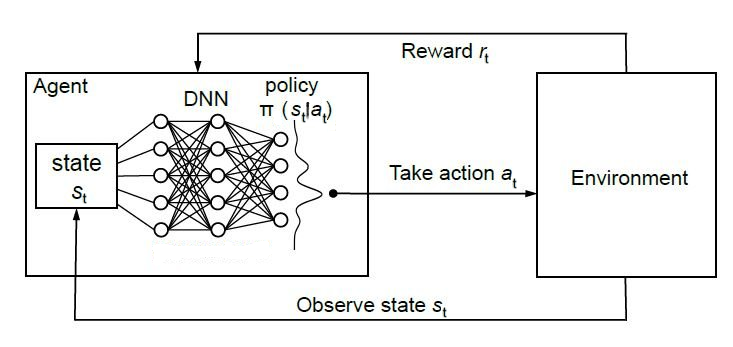
\includegraphics[width=0.85\textwidth]{pic/1}
    \caption{Взаимосвязь агента и среды[2]}
    \label{fig:img1}
\end{figure}

Задача агента — максимизировать expected return:

\begin{equation}
    J(\pi)=E_{\tau\sim\pi}[R(\tau)]=E_{\tau\sim\pi} \left[\sum_{t=0}^n r_t\right]. [2]
\end{equation}

Таким образом математически задачу RL можно сформулировать как поиск такой оптимальной стратегии $\pi^*$, что $\pi^* = arg \mathop {max} _ \pi J(\pi)$[2].

Таким образом можно сделать вывод, что обучение с подкреплением полностью завязано на взаимном воздействии агента и среды вне зависимости от алгоритма.
О такой системе говорят, что она имеет обратную связь, поэтому ее нужно рассматривать как единое целое, из-за чего линия разделения между средой и агентом
в этой системе достаточно условна. Эта взаимосвязь схематично показана на рисунке 5. Эта взаимосвязь рассматривют как последовательность пар state и
reward, переходами в которые являются actions агента:

\begin{equation}
    (s_0) \stackrel{a_0}{\rightarrow} (s_1, r_1) \stackrel{a_1}{\rightarrow} ... \stackrel{a_{n-1}}{\rightarrow} (s_n, r_n). [2]
\end{equation}

\section{Задачи, решаемые с помощью обучения с подкреплением}
Обучение с подкреплением применяется там, где принятое решение может иметь последствия не только сразу после его принятия,
но и спустя некоторый промежуток времени. Поэтому алгоритмам данного вида обучения иногда приходится ждать, чтобы
увидеть последствия своих решений. Обычно даже человеку в таких задачах сложно понять, какой порядок действий приводит к
какому результату.

К таким задачам относятся:
\begin{enumerate}
    \item Создание продвинутого ИИ для игр. Сейчас большинство ИИ в играх создаются на основе математических автоматов с множеством состояний
    и переходов. Однако этот подход является не самым совершенным, и поэтому качество такого ИИ оставляет желать лучшего. Подход же с нейросетью,
    обученной с помощью RL, является более совершенным. Так такие ИИ могут спокойно обыгрывать чемпионов мира по шахматам или представлять реальную
    угрозу даже самым умелым игрокам. Ярким примером является OpenAI Five. [3]
    \item Обучение модели для автономного вождения. Изначально моделируется несколько различных сред для машины, которая в данном случае является агентом,
    а затем в них по очереди помещается сам агент для обучения на всех возможных ситуациях. Так сначала модель обучется на пустой дороге, чтобы модель понимало,
    что агент должен ехать только по ней по ней, затем агента запускают в среду с пешеходами и знаками дорожного движения, чтобы научить модель соблюдать ПДД,
    а после его начинают запускать в среды, которые представляют из себя различные специфичные ситуации: зимние дороги, непогоду, ремонтные работы, поломанные
    дороги и т.д. Ярким примером использования алгоритмов RL в данной сфере являются машины компании Tesla. [1]
    \item Обучение роботов в робототехнике. Схоже с предыдущим пунктом, меняются лишь цели обучения, возможности действий агента, условия самих сред и их количество
    в зависимости от самой задачи. [1]
    \item Чат боты, основанные на нейронных сетях. Для данной задачи существует несколько подходов. Первый из них представляет из себя создание огромного ансамбля
    NLP (Natural Language Processing) моделей, работающих как параллельно, так и последовательно. Второй же завязан на одной модели, обученной с подкреплением. В
    этом случае средой выступают диалоги с обычным пользователем, а агентом сам чат бот. [4]
    \item Рекомендательные системы. Данный класс задач тоже можно решать с помощью RL. Тогда выдача рекомендации того или иного предложения будет являтся действием в среде,
    а средой будет выступать совокупность того место, где будет появятся рекомендация и людей, находящихся в данной среде. Этот подход в преспективе является лучше
    классического двухуровневого подхода к данной задаче, однако проигрывает ему в скорости обучения, потому что в двухуровневом подходе обучение происходит
    перед использованием модели, за счет чего мы получаем неплохое качество рекомендаций уже после добавления такой функции, а RL моделью обучается при 
    взаимодействие с ней пользователей. [5]
\end{enumerate}

\section{Алгоритмы RL}
\subsection{Наивные подходы}
Самый постой подход к данному классу очень просто и не предполагает использование ИНС. Его реализация представляет собой использование динамического программирования и
состоит из двух шагов:
\begin{enumerate}
    \item Перебрать все возможные стратегии.
    \item Найти самую оптимальную стратегию, дающую наибольшую награду.
\end{enumerate}
Главная проблема такого подхода - это количество стратегий, которые надо обработать. Их количество может быть не просто очень велико, а бесконечно. Вторая проблема
заключается в плохом обобщении такой системы. Использование ИНС хорошо решает эти проблемы, не рассматривая все стратегии, а выбирая, основываясь на своем опыте
предыдущем опыте, оптимальную.

Данную задачу можно также попробовать решить стандартными алгоритмами, обучая их с подкреплением, однако такое решение не принесет нужный результат вне зависимости от сложности модели.
Так происходит по одной простой причине, которая заключается в дизбалансе классов, вызванный случайными действиями агента в ситуациях, в которых он не знает как действовать,
из-за чего некоторые действия могут вовсе не воспроизводиться. Более простыми словами полезные сигналы теряются на фоне шума, который обусловлен редкими наградами. Поэтому для
задач RL используют специальные алгоритмы. Список таких алгоритмов можно увидеть на рисунке 7.

\begin{figure}[H]
    \centering
    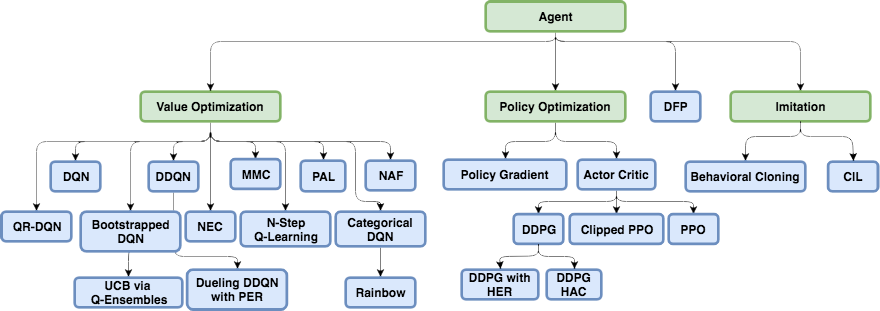
\includegraphics[width=0.85\textwidth]{pic/2}
    \caption{Алгоритмы RL[6]}
    \label{fig:img1}
\end{figure}

\subsection{Q-learning}
Раньше, когда НС не существовало, а мощностей компьютера не хватало для высоконагруженных вычислений, уже существовал RL. Он выглядил как простая, но очень оригинальная идея:
делать случайные действия, а потом для каждой ячейки в таблице и каждого направления движения, посчитаем по формуле уравнения Беллмана (6) насколько хороша эта ячейка и выбранное направлени. Чем
выше это число, тем с большей вероятностью этот путь ведет к большей выгоде. Само такое число получило название Q (от слова quality — качество выбора, очевидно), а метод —
Q-learning.
\begin{figure}[H]
    \centering
    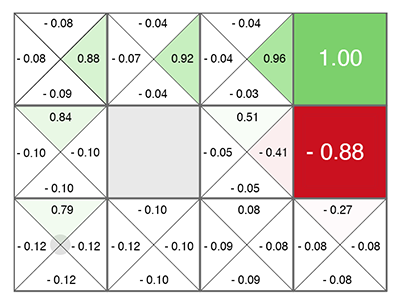
\includegraphics[width=0.65\textwidth]{pic/3}
    \caption{Пример табличного RL[6]}
    \label{fig:img1}
\end{figure}
Чтобы побороть проблему обычных ИНС, описанную выше ученые вернулись к классическому табличному Reinforcement Learning, но вместо ручного подсчета значений таблицы в качестве
целевой функции стали использовать НС. На основе этого подхода и строятся алгоритмы RL сегодня и, он же является отличием от обычного обучения нейросетей. Классический же
алгоритм, в основе которого лежит только заполнение таблицы получил название DQN (Deep Q-learning Network)[20].

В DQN на вход нейросети подается текущая ситуация (state), а на выходе нейросеть предсказывает число Q. А так как на выходе сети перечислены сразу все возможные действия
(каждый со своим предсказанным Q), то получается что нейросеть в DQN реализует классическую функцию Q(s,a) из Q-learning. Следовательно для получения самого оптимального
действия в заданной ситуации нужно использовать argmax, для который вернет индекс действия с максимальным Q. Такая политика будет называться детерминистской. Но более
оптимальной будет стохастическая политика. При ней выбирается случайное действие з доступных, но пропорционально их Q-значениям (т.е. действия с высоким Q будут выбираться
чаще, чем с низким). Такая политика является более оптимальной, так как она выбирает действия, которые в данный момент могут не нести особого смысла в данный момент, но могут
в дальнейшем привести к действиям с большей наградой и меньшим штрафам.

Главый минус такого алгоритма, что он работает только с агентом, который может совершать небольшое количество детерминированных действий (при их высоком количестве метод просто не сходится).
Чтобы решить данную проблему были придуманы другие алгоритмы, оптимизатором для которых стал модифицированный алгоритм градиентного спуска, получивший название Policy Gradient.

\subsection{Policy Gradient}
Идея алгоритма очень проста: подавать на вход НС текущее состояние, на выходе сразу предсказывать действия $\pi_\theta(a_t|s_t)$, а затем сравнивать полученную награду за действие
со средней наградой. Таким образом по динамике $R(\tau) = \sum_{t=0}^T r_t$ становится возможно вычислять вектор градиент. Эта модификация позволяет свести задачу обучения RL сети к
обычной задачи классификации, следовательно в качестве функции потерь можно использовать модифицированную версию кросс-энтропии:
\begin{equation}
    loss = -log(\pi_\theta(a_t|s_t))R(tau). [2]
\end{equation}
За счет этого происходит уменьшение шума, который не давал корректно обучать классические модели НС для класса задач RL.

Преимуществом данного метода является возможность обучать модель с большим количеством действий, а также гибкая система поощрений и наказаний. К минусам же можно отнести
то, что пересчет весов модели происходит только в конце эпохи, а не с каждым шагом агента.[7]
\subsection{Actor-critic}
Следующая модификация, которая была добавлена в алгоритмы RL, это добавление явного учителя, который представляет из себя новую модель, которая будет оценивать действия
агента. Такую модель называют критиком, а агента - актером.

Актерская модель практически ничем не отличается от стандартной архитектуры агента. На вход так же подается состояние среды в данный момент и на выход выдается действия
или вектор вероятностей уместности действий в данной ситуации.

Критическая модель получает на вход так же получает состояние и действие, предсказанное первой моделью, а на выход ввыводет значение значению $Q$, которое будет
являться функцией от входных параметров $Q(s, a)$.Таким образом за счет оценки критика обучается актер на основе Police Gradient, а критик будет учится обычным
путем, согласно с реальным прохождением эпизода.

Примером алгоритма использующего классическую реализацию Actor-critic является DDPG. Более продвинутые модели способны сравнивать новую политику с предыдущей
и на основе этого корректировать свои веса. В этом случае для рассчета градиента используется не просто функция $Q(s,a)$, а $A(s,a) = Q(s,a) - V(s)$.[2] В данном случае
функция $A(s, a)$ как раз и показывает насколько после предпринятых действий станет лучше, чем текущая ситуация $V(s)$(в самой простой реализации $Q(s,a)$ можно
заменить на $r$ и таким образом $A = r - V(s)$). Примером таких алгоритмов являются A3C/A2C. Их главным минусом является резкое изменение весов моделей из-за чего
процесс спуска становится более стохастическим, поэтому более поздние алгоритмы, такие как Proximal Policy Optimization (PPO)[7] и Trust Region Policy Optimization (TRPO)[7]
имеют ограничению на изменение весов (что-то вроде gradient clipping в рекуррентных сетях для защиты от взрывающихся градиентов, только на другом математическом аппарате),
один из которых и используется в практической части данной работы.

\section{Оценка качества обучения с подкреплением}
По завершении процесса обучения, критически важно оценить эффективность модели. Для этого применяются специализированные метрики
качества. Разнообразие существующих метрик позволяет подходить к различным задачам уникальным образом, учитывая разные аспекты
каждой модели. Следовательно, выбор наиболее подходящей метрики для конкретной задачи играет ключевую роль в оценке успешности обучения
модели.

Вот некоторые из наиболее распространенных метрик для оценки качества обучения с подкреплением:

\begin{enumerate}
    \item Суммарное вознаграждение (Total Reward): Это основная метрика в обучении с подкреплением, измеряющая общую сумму вознаграждений, полученных агентом за эпизод или серию действий. Она отражает общую эффективность стратегии агента;
    \item Среднее вознаграждение за шаг (Average Reward per Step): Эта метрика измеряет среднее вознаграждение, получаемое агентом за одно действие. Она полезна для оценки эффективности агента в каждом конкретном действии;
    \item Сходимость (Convergence): Эта метрика оценивает, насколько быстро политика или стратегия агента сходится к оптимальному решению. Быстрая сходимость обычно желательна, так как она указывает на эффективное обучение;
    \item Вариабельность вознаграждения (Reward Variability): Эта метрика измеряет стабильность вознаграждений, получаемых агентом. Низкая вариабельность указывает на то, что агент последовательно выполняет хорошие действия;
    \item Процент успешных эпизодов (Success Rate): Для задач, где есть четко определенный критерий успеха, эта метрика измеряет долю эпизодов, в которых агент достигает цели;
    \item Энтропия политики (Policy Entropy): Эта метрика используется для измерения степени случайности в действиях агента. Высокая энтропия может указывать на то, что агент исследует различные стратегии, в то время как низкая энтропия может указывать на сильно детерминированное поведение;
    \item Оценка времени до достижения цели (Time to Goal): Эта метрика измеряет, сколько времени требуется агенту для достижения определенной цели или задачи.[8]
\end{enumerate}

\begin{thebibliography}{3}
    \bibitem{1}
    Катрина Уэйкфилд "Гид: алгоритмы машинного обучения и их типы" [Статья] – URL: https://www.sas.com/ru_ru/insights/articles/analytics/machine-learning-algorithms-guide.html (дата обращения 10.01.2024) - Загл. с экрана. Яз. рус.
    \bibitem{2}
    Документация PyTorch [Электронный ресурс] – URL: https://pytorch.org/ (дата обращения 12.01.2024) Яз. англ.
    \bibitem{3}
    OpenAI Five [Электронный ресурс] – URL: https://openai.com/five/ (дата обращения 12.01.2024) - Загл. с экрана. Яз. англ.
    \bibitem{4}
    D. Biswas "Self-improving Chatbots based on Deep Reinforcement Learning" [Статья] – URL: https://towardsdatascience.com/self-improving-chatbots-based-on-reinforcement-learning-75cca62debce (дата обращения 13.01.2024) - Загл. с экрана. Яз. англ.
    \bibitem{5}
    M. Berk "How to Use Reinforcement Learning to Recommend Content" [Статья] – URL: https://towardsdatascience.com/how-to-use-reinforcement-learning-to-recommend-content-6d7f9171b956 (дата обращения 13.01.2024) - Загл. с экрана. Яз. англ.
    \bibitem{6}
    Что не так с обучением с подкреплением (Reinforcement Learning)? [Электронный ресурс] – URL: https://habr.com/ru/post/437020/ (дата обращения 13.01.2024) - Загл. с экрана. Яз. рус.
    \bibitem{7}
    Intro to Policy Optimization [Электронный ресурс] – URL: https://spinningup.openai.com/en/latest/spinningup/rl_intro3.html (дата обращения 13.01.2024) - Загл. с экрана. Яз. англ.
    \bibitem{8}
    Evaluation metrics for reinforcement algorithms [Электронный ресурс] – URL: https://medium.com/@barathchandarcse/evaluation-metrics-for-reinforcement-algorithms-ff2bf5869fe4 (дата обращения 13.01.2024) - Загл. с экрана. Яз. англ.
\end{thebibliography}


\end{document}